\chapter{Cores and Flashing}
\label{cha:cores}

\phantomsection
\section{What are cores, and why does it matter?}

The MEGA65 computer uses a versatile chip called an FPGA as its heart.
FPGAs are ``Field Programmable Gate Arrays''. This is a fancy way of
saying that FPGAs are chips that can be programmed to behave impersonate
other chips.  They do this by configuring their arrays of logic gates to
reproduce the circuits of other chips. In this way, FPGAs are not emulation
but re-creation of other chips.

FPGAs forget what chip they were pretending
to be whenever the power is turned off, or when they are ``reconfigured''.
This might sound annoying, but it's actually really powerful. It means that
we can tell the FPGA in the MEGA65 to impersonate not just the MEGA65 design
as it currently stands, but to impersonate any improvements we make to the design.
In other words, we can upgrade the MEGA65 hardware just by providing a new
set of instructions to the FPGA.  These sets of instructions are called ``cores''
or ``bitstreams''.  For the purpose of the MEGA65, these two terms can usually be
considered to be interchangeable.

FPGAs are so flexible, that not only is it possible to teach the MEGA65 to be a better
MEGA65, but it is also possible to teach the MEGA65's' FPGA to be other interesting
home computers.  We believe that the FPGA is powerful enough that it could pretend to be
a VIC-20 (tm), Commodore PET (tm), Apple II (tm), Spectrum (tm), BBC Micro (tm), or even
an Amiga (tm) or one of the 16-bit era game consoles.  Unlike some previous FPGA-based
retro-computers, the MEGA65, its FPGA instructions, board layout and other information is
all available for free under open-source licenses. This means that anyone is free to
create other cores for the MEGA65 hardware.

To top it all off, the MEGA65 has enough storage for 7 different sets of FPGA instructions,
so that you can easily switch the MEGA65's ``personality'' from being a MEGA65 to another
of these systems (once the cores are available) and back again.

The remainder of this chapter describes how to select which core to run on the MEGA65, and
how to store a core into one of the seven slots in the flash memory storage.

\phantomsection
\section{Selecting a core}

To operate the MEGA65 using an alternative core, turn off the power to the MEGA65, and then hold the
\megakey{TAB} key down while turning the power back on.  This instructs the MEGA65 to enter the
flash and core menu, instead of booting normally.  You should see a display like the following:

XXX - Screen shot of flash menu with 7 empty slots.

To select a core and start it, use the cursor keys to highlight the desired core, and then press the
\megakey{RETURN} key.  Alternatively, you can press the number corresponding to the core you would
like to use. The MEGA65 immediately reconfigures the FPGA, and launches the core.  If for some reason
the core is faultly, the MEGA65 may instead restart normally after a few seconds, and depending on the
circumstances, take you automatically back into the menu.

The MEGA65 will keep running the new core until you physically power it off.  Pressing the reset button
will not reset which core is being run.

\phantomsection
\section{Installing an upgrade core for the MEGA65}

To install an upgrade core for the MEGA65, there are few easy steps.

First, copy the core file onto the MEGA65's SD card.  You can do this by removing the SD card and inserting
it into another computer that has internet access, and downloading the core from that computer. Alternatively
you can insert an SD card that already contains the upgrade core. Finally, you can use the MEGA65 TFTP Server
program and the MEGA65's ethernet port to copy the core upgrade file onto the SD card from another computer
on your local network.

Second, once you have the upgrade core on the MEGA65's SD card, enter the flash and core menu as above,
i.e., turn off the power, hold the \megakey{TAB} key down while turning the power on.  When the flash
and core menu appears, hold the \megakey{CTRL} key down and press the \megakey{1} key.  The MEGA65
will present you a list of core files that are on the SD card.  Select the upgrade core file you wish to
install using the cursor keys, and then pressing the \megakey{RETURN} key.  The MEGA65 will then erase
the flash slot, before writing the upgraded core.  This process is quite slow, and can take around 15
minutes.

It is important to not turn the power off during this process. If you do, the core file will be
only partially installed, and the MEGA65 may not start properly. If this happens, enter the flash and core
menu as described above, and follow the instructions again.  When the process completes, you will see a message
like this, indicating that the process is complete:

XXX

When this happens, simply turn off the power to the MEGA65 and turn it back on for it to start using the
upgraded core.  This is because the MEGA65 will always try to automatically start the core in slot 1 when
it is turned on.

\phantomsection
\section{Installing other core for the MEGA65}

Installing other cores works very similarly to installing upgrade cores. The only difference is that you
press \megakey{CTRL} and \megakey{2} to \megakey{7} from the flash and core menu, so that the core
gets installed in another slot.

Of course, there is nothing stopping you installing a different core
in slot 1, so that the MEGA65 behaves as a different type of computer when you turn it on.  If you do this,
you can always choose to run the MEGA65 core by entering the flash and core menu,  and selecting the MEGA65
core.

\phantomsection
\section{Creating cores for the MEGA65}

If you would like to create your own cores for the MEGA65, or help contribute to the MEGA65 core, then
you may also wish to take a look at Appendix \ref{cha:fpgacpldflashing} which explains how to use the
FPGA development tools to flash the MEGA65.

\phantomsection
\section{Replacing the factory core in slot 0}

Replacing the core in slot 0 is not recommended, because if you mess it up, it will brick the machine.
This may require that you have to purchase a TE-0790 JTAG programmer, open your MEGA65 case, install
the module, go through some rather convoluted software preparation steps, similar to if you were
creating your own bistream/core, and then restore a working bitstream into the slot.

The MEGA65 is an open system though. Therefore we have not made it impossible for you to do this,
just very hard: There
is a secret key press in the flash menu that will then challenge you with a series of questions of
increasing difficulty, to ensure that you know what you are doing.  Only after you have correctly
answered these questions, will you be given the option to erase and/or replace the contents of slot 0.
We are purposely not documenting the method for doing this, nor further details of the questions
you will be asked.

However, there really should be no reason for using this method to replace the contents of slot 0:
If you want to make your own bitstreams/cores, you can either put them in other slots, and use the
flash menu to activate them, or you should simply use a TE-0790 JTAG adapter, and then use
the Vivado or other FPGA development tools to write to the flash directly.  That method is also
somewhat faster than flashing through the flash menu.

You have been warned!

\phantomsection
\section{Understanding The Core Booting Process}

This section summarises how the MEGA65 selects which core to start when it is powered on.
The process is as shown in the following figure: When the MEGA65 is
powered on, it always starts the bitstream stores in slot 0 of the
flash.  If that is the MEGA65 Factory Core, the MEGA65 HYPPO
Hypervisor starts.  If it is the first boot since power-on, HYPPO
starts the Flash Menu programme -- but note that the Flash Menu in
this mode may not show anything on the screen to indicate that it is
running!

The Flash Menu checks if the system is booting from Flash
Slot 0.  If it is, it checks if the NO SCROLL key is being held.  If
it is, the Flash Menu programme shows its display, allowing the user
to select or re-flash a core. If the NO SCROLL key is not being
pressed, then the Flash Menu programme checks if Flash Slot 1 contains a valid
core.  If it does, then the Flash menu programme attempts to start
that core.  If it succeeds, then the system reconfigures to that core,
after which the behaviour of the system is according to that core. If
it fails, the keyboard will show the flashing red and blue ``ambulance
lights'' to indicate that some first-aid is required.  Note that in
the ambulance light mode that the reset button has no effect: You must
turn the computer off and on again.

If the user selected a different core in the Flash Menu, the process
is similar, except that the ambulance lights will appear for only a
limited time, as the FPGA will automatically search through the flash
memory until it finds a valid core. If it gets to the end of the flash
memory, it will start the MEGA65 Factory Core from slot 0 again.

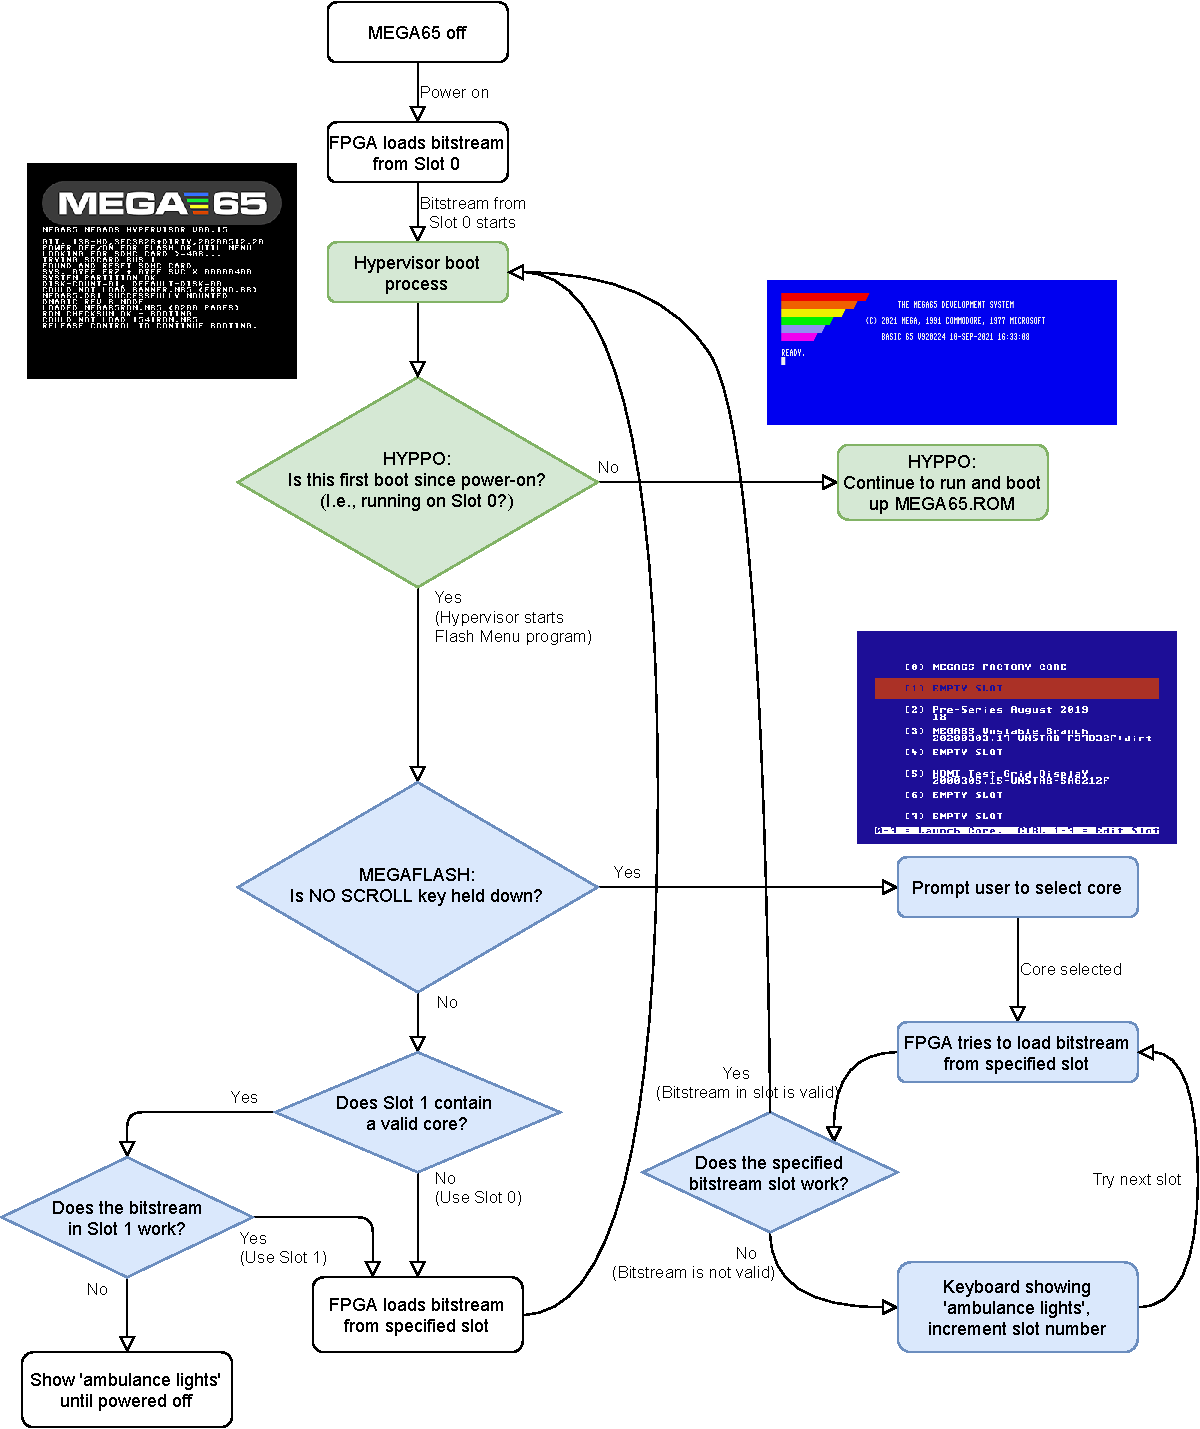
\includegraphics[width=\linewidth]{images/illustrations/flashmenu-flowchart.pdf}


